%!TEX root = ../main.tex

\section{More Shortest Paths}

\subsection{Dijkstra's Algorithm}

\subsubsection{High Level Overview}

Recall we are trying to find the single source shortest path in a directed, weighted graph $G = (V, E)$ from the source $s$ to all vertices. For this problem we will assume all weights are non-negative.

\begin{definition}
    We say the length of a path is the sum of the weights of all the edges going through that path.
\end{definition}

Consider the single source $s \in V$. The shortest path from $s$
to itself is 0. Think of this as the base case for the inductive
procedure. For the inductive step, partition $V$ into $S$, which we
call the source side, as the set of
vertices for which we know the shortest path from $s$, and $V - S$,
as the rest of vertices for which we don't know the shortest path from
$s$. The idea is to grow $S$ until $S = V$. Initially,
$S = \{s\}$, $d(s) = 0$, and $d(v) = \infty$ for all other vertices.

\begin{definition}
    A path from $s$ that stays entirely within $S$ will be
called a source-side path.
\end{definition}

At each stage find the vertex $v \in V - S$ for which there is a
vertex $u \in S$ such that the $d(s, u) + w(u, v)$ is minimum over all
$x \in V - S$. Then add $v$ to $S$ and update appropiately. As you may
have noticed, this is a greedy algorithm.

\subsubsection{Details}

For each vertex $v$, maintain a quantity called $d(v)$. For vertices
in $V - S$, $d(v)$ is the length of the shortest path from $s$ to $v$
consisting of a source side path to some vertex $u \in S$ followed by
the edge $(u, v)$ (see Figure~\ref{fig:dijkstra}).

\begin{figure}[hpt]
    \centering
    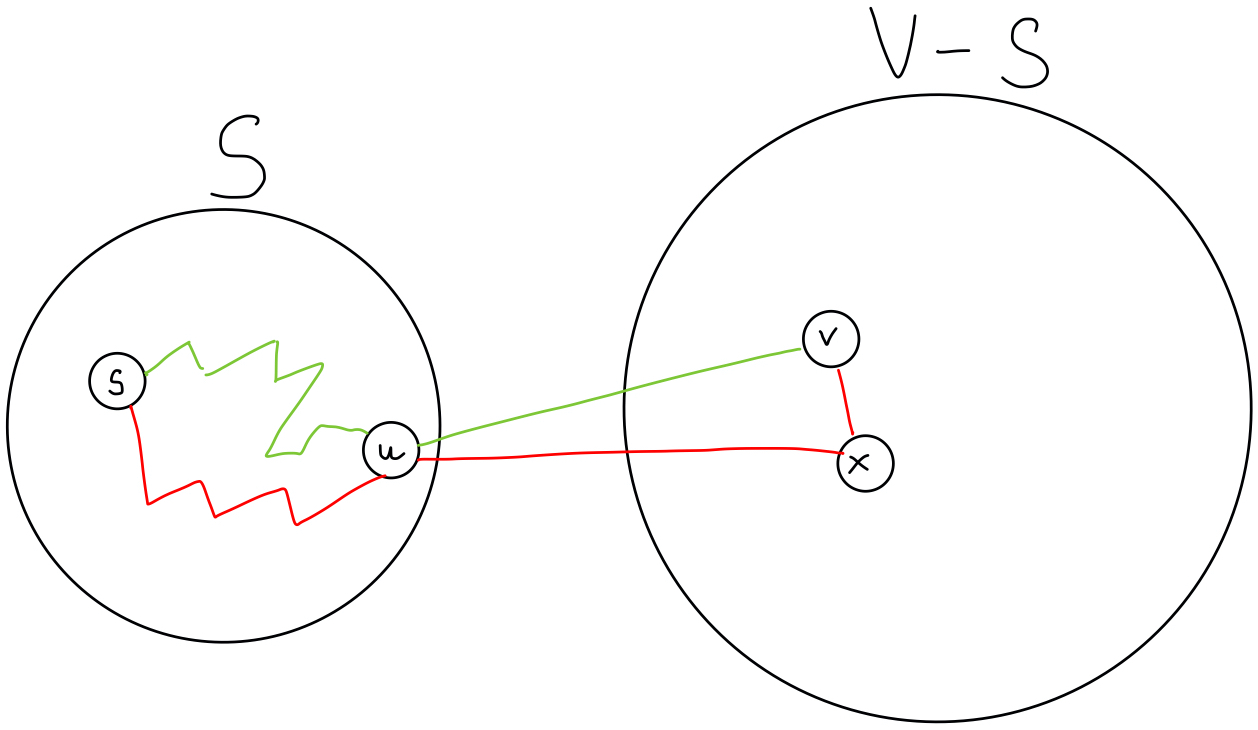
\includegraphics[width=0.5\textwidth]{figures/dijkstra.jpeg}
    \caption{The green path is a form we allow $d(v)$ to be in, while
    the red path is a form we don't allow, as we had an intermediate
    $x \in V - S$ before our final $v$.}
    \label{fig:dijkstra}
\end{figure}

At each iteration, we bring the vertex $v \in V - S$ with minimum 
$d(v)$ to $S$. Then, for each neighbor $x$ of $v$, we update $d(x)$ to
be

$$
d(x) = \min(d(x), d(v) + w(v, x))
$$

\subsubsection{Proof of Correctness}

The correctness of this algorithm relies on Theorem~\ref{thm:dijkstra}.

\begin{theorem}\label{thm:dijkstra}
    For each vertex $v \in S$, $d(v)$ is equal to the shortest
    path from $s$ to $v$.
\end{theorem}

\begin{proof}
    By induction. In the base case, after the first iteration,
    $S = \{s\}$ and $d(s) = 0$, which is correct. Assume for the
    inductive hypothesis that the statement is true for
    $|S| = k$, and suppose $v$ is the $k+1$th vertex brought into $S$.
    Recall $v$ is brought into $S$ because $d(v)$ is minimum. Let
    $P$ be the path with length $d(v)$. For a contradiction, suppose
    there is a shorter path $P'$ to $v$. We know $P'$ must include
    one edge from $S$ to $V - S$, so let $(x, y) \in E$ be such edge,
    where $x \in S$ and $y \in V - S$.
    Then $(s, y)$ portion of $P'$ is at least as long as $P$ by the
    way our algorithm works, and therefore $P'$ is at least as long as
    $P$. This proves that at the point the algorithm brings $v$ into
    $S$, $d(v)$ is the length of the shortest path to $v$. 
\end{proof}

\section{Huffman Coding}

Suppose you have a text over a large alphabet (say an English text).
When you transmit this text over a network, you need to encode the
text in binary for storage and communication. Therefore, it would be
nice to encode this with the fewest bits possible.

We're only interested in the following restricted problem. The code
has to be a mapping from the symbols in the original alphabet $\Sigma$
to binary strings, and the decoding has to be unambiguous. For
instance, if our alphabet is $A, B, C, D$ with mapping
$A \to 01$, $B \to 011$, $C \to 100$, and $D \to 00$, then the binary
string 01100 can either be $BD$ or $AC$. We don't want that!

Furthermore, if one word is a prefix of another, this could lead to
ambiguity, so our code has to be prefix free. 

\begin{definition}
    Codes that are prefix free are called prefix codes.
\end{definition}

An example of a code is ASCII. This is not very efficient, as every
letter in the alphabet has a mapping to a bitstring that is the same
size as the rest. Naturally, we would like frequent letters in a text
to have a shorter bitstring and letters that occur unfrequently to
have a longer bitstring.

Let $\Sigma = \{\sigma_i, \sigma_2, ..., \sigma_n\}$, and let
$f_i$ be the frequency of $\sigma_i$. You can think of these
frequencies as probabilities so that $\sum_i f_i = 1$. The goal is
to find a prefix code that maps $\sigma_i$ to $c(\sigma_i)$ that
minimizes $\sum_i f_i |c(\sigma_i)|$, which is the average code length.

A binary code can be thought of as a binary tree. For instance, for
$A \to 00$, $B \to 010$, $C \to 011$, and $D \to 1$, we have that the
binary tree is Figure~\ref{fig:huffman}.

\begin{figure}[hpt]
    \centering
    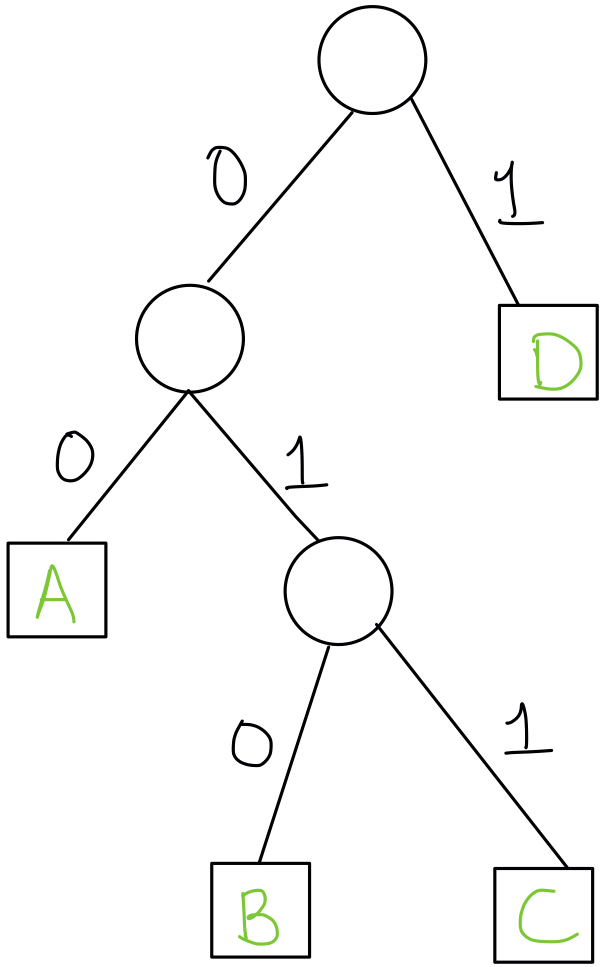
\includegraphics[width=0.3\textwidth]{figures/huffman.jpeg}
    \caption{Example Huffman Coding}
    \label{fig:huffman}
\end{figure}

\begin{definition}
    A full binary tree is a tree where every internal node has two
    children.
\end{definition}

Notice symbols are at the leaves for a prefix code. Also, the tree
corresponding to an optimal code must be a full binary tree. For if the tree is not a full binary
tree, there must be an internal node $v$ with only one child. But then
$v$ is redundant and you can remove $v$.

Suppose we know the shape of the optimal tree (which is a full binary
tree).

\begin{lemma}
    Any full binary tree has a pair of sibling leaves at the deepest
    level.
\end{lemma}

\begin{proof}
    Look at a leaf at the deepest level. Look at its parent. By
    definition of a full binary tree, the parent must have two
    children. So the leaf has a sibling.
\end{proof}

\begin{lemma}
    In the optimal tree, the two symbols of least frequency are at the
    deepest level of the tree.
\end{lemma}

\begin{proof}
    By exchange argument. Suppose $x$ and $y$ are the
two symbols with least frequency, and suppose that the two leaves at
the deepest level have symbols $a$ and $b$, where $\{a, b\} \neq 
\{x,y\}$. By exchanging positions of $a$ with $x$ and $b$ with $y$
we can bring $x$ and $y$ to the deepest level. One can show using
simple algebra that this is an improvement (exercise: show it).
\end{proof}

Suppose you have two symbols $x$ and $y$ at depth $d + 1$ which are
siblings in the binary tree. Construct a new symbol $xy$ in place of
$x$ and $y$ that
is going to be the parent of $x$ and $y$ with depth $d$. 
We know $f(xy) = f(x) + f(y)$, and if you look at the contribution of
$x$ and $y$ to the average code length, we have that they contribute
$(f(x) + f(y))(d+1) = f(xy)(d+1)$, where $d + 1$ is the depth of $x$
and $y$. However, the contribution that $xy$ makes to the average
code length is $f(xy)d$. Therefore, the same tree with this new symbol
has cost $f(xy)$ lower.

\subsubsection{Huffman's Algorithm}

(Sketch) Combine the two least frequent symbols $x$ and $y$ into one
symbol $xy$ with frequency $f(xy) = f(x) + f(y)$. Recursively solve
the problem on $n - 1$ symbols, since Huffman's coding has optimal
substructure.




